\textbf{Reinforcement learning (RL)} is an area of machine learning that epitomizes the agent-based approach.
RL is unique within this field as it is directly focused on goal-directed learning from agent-environment interaction \cite{rlai}.
At the core of RL is the \emph{reward function}, which perfectly describes goals established by the problem.

RL is a class of problems as well as a class of solutions to those problems \cite{rlai}.
Despite the apparent \emph{supervised-unsupervised} split in machine learning, RL is cannot entirely fit in neither subset \cite{rlai}.

In the following chapter, we present the main concepts forming the framework of reinforcement learning.

\section{Feedback Loop}
First of all, we present the feedback loop, central to understanding the RL dynamic.
This is just a reiteration of the contents in our previous chapter:
an agent acts upon the environment, which reacts according to its set of governing rules.
The novel concept here is the \emph{reward signal}.
\begin{enumerate}
    \item The agent is in state \(s\) and picks action \(a\).
    \item It receives a reward \(r\) for its action. This (immediate) reward signal is problem-defined and quantifies the agent’s goal.
    \item The environment reacts, sending the agent into the next state \(s'\).
    \item The agent perceives \(s'\) and needs to decide on its next action.
\end{enumerate}

\begin{figure}[ht]
    \caption{The feedback loop in reinforcement learning. (Partial reproduction from \cite{rlai}, 3.2)}
    \centering
    \vspace*{0.5cm}
    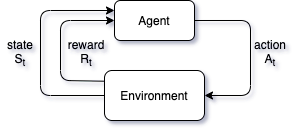
\includegraphics[width=0.5\textwidth]{agent-env-fig}
\end{figure}

Besides agent, reward and environment, we need to introduce several new concepts. A RL agent can be decomposed into state, policy, value function and (optionally) model \cite{rlai}.

\section{State and Policy}

The \textbf{state} most often refers to the internal state of the agent.
Although, in some contexts, we can use it to mean the environment state.
A state contains relevant information from the environment at a given time-step.
A key point in RL is that a well-engineered (agent) state captures all the relevant information and removes the need of explicitly memorizing state history.
This is mathematically by described the \textbf{Markov property} \cite{silver-lectures}, a fundamental property of the mathematical framework underpinning RL -- Markov decision processes (MDPs).

A \textbf{policy} completely characterizes the agent’s behaviour.
``It is a mapping from perceived states of the environment to actions to be taken in those states'' \cite{rlai}.
Policies can be deterministic (i.e. ``if this then that'' rules) or stochastic.
A \textbf{stochastic policy}\cite{silver-lectures} is a probability distribution over actions, given a state.

\section{Reward}
``The reward signal is the primary basis of altering the policy.'' \cite{rlai}.
The \textbf{reward} models the problem-defined goals as a scalar that can be associated with each state transition.
The assertion that we can completely and correctly model all goals using reward functions is central to the field of RL.
This is called the \textbf{Reward Hypothesis} and is formulated below:
\begin{quotation}
    That all of what we mean by goals and purposes can be well thought of as maximization of the expected value of the cumulative sum of a received scalar signal (called reward). \textit{(from \cite{rlai}, Chapter 3.2)}
\end{quotation}

The \textbf{return} denotes the cumulative reward obtained by the agent over time.
This is what a RL system is supposed to maximize.
There are multiple mathematical models used to represent the return.
The simplest example is to simply sum the reward over a finite number of steps.
However, in practice we often use \textbf{discounting}.
Discounting is, simply, a way to control how much the agent cares about future rewards.
More on this topic can be found in either theorethical reference \cite{rlai,silver-lectures}.
% In the actual paper, elaborate here.

\section{Value Function}\label{rl:value-func}

A \textbf{value function} measures how good each state is, with regard to the long-term potential of that state.
``Whereas rewards define the immediate desirability of an environmental state'', a value function ``indicates the long-term desirability of a state'' \cite{rlai}.
The value of a state is given by two things:
\begin{enumerate}
    \item the immediate value of being in that state (that state’s immediate reward)
    \item the potential return going forward in time from that state.
\end{enumerate}

This models a \textbf{long-term thinking aspect} into learning, as choosing one state over another often excludes future paths of action.
Let us take a game of chess as example.
If one move leads to the opponent capturing one of the agent's pieces, no future actions can be executed with that piece.
Thus, making a move with a high initial reward (for example, the agent trades a pawn for a knight), excludes -- for example -- the option of \textbf{promoting} that particular pawn (a later, higher reward).

\section{Model}
A RL system may or may not have a \textbf{model}.
A \textbf{model} (of the environment) allows the agent to plan and make predictions of its environment.

Some algorithms focus explicitly on learning a model and use it for \emph{planning}.
This approach is called \textbf{model-based}.
In this case, an agent can query the model to simulate what would happen with the environment, before actually choosing an action (hence the planning aspect).

Approaches without a model are called \textbf{model-free}.
Model-free agents are ``explicitly trial-and-error learners'' \cite{rlai}.

\begin{figure}[ht]
    \caption{A way of classifying RL methods based on whether they have a value function, policy or model. (Reproduced from David Silver's lectures. \cite{silver-lectures})}
    \vspace*{0.2cm}
    \centering
    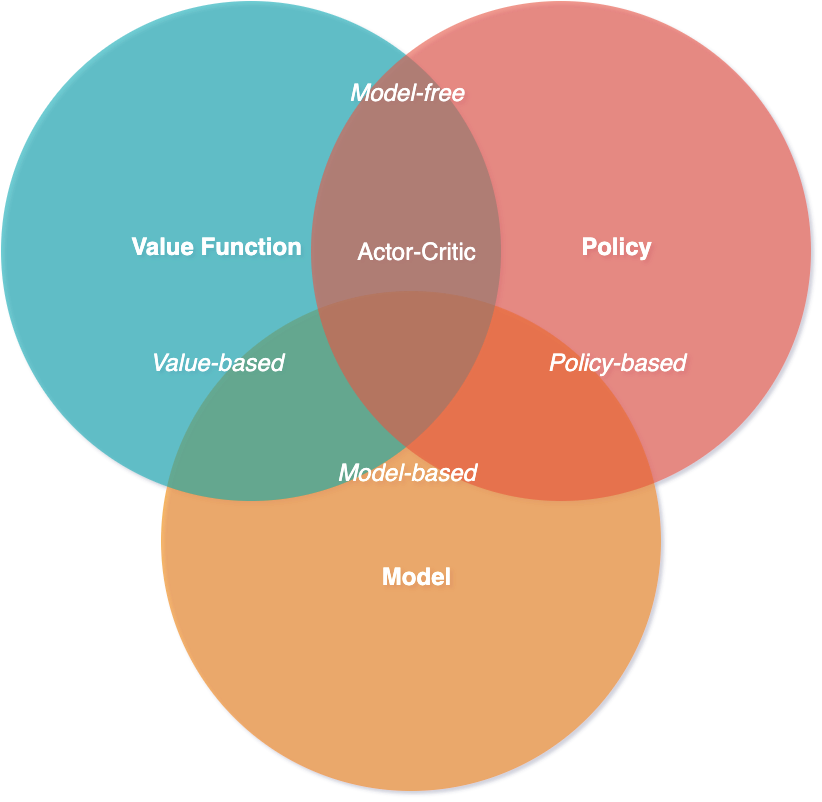
\includegraphics[width=0.5\textwidth]{silver-venn}
\end{figure}
